\documentclass[a4paper,12pt]{report}
\usepackage[romanian]{babel}
\usepackage{blindtext}
\usepackage{amsmath}
\usepackage[utf8]{inputenc}
\usepackage[left=3cm, top=2cm, right=2cm, bottom=2cm]{geometry}
\usepackage{titlesec}
\usepackage{graphicx}
\newcommand\tab[1][1cm]{\hspace*{#1}}
\titleformat{\chapter}[display]
{\normalfont\large\bfseries\centering}{\chaptertitlename\ \thechapter}{0pt}{\Huge}
% this alters "before" spacing (the second length argument) to 0
\titlespacing*{\chapter}{0pt}{0pt}{20pt}

\begin{document}

\begin{titlepage}
	\begin{center}
	\centering
	{\scshape\LARGE Universitatea din București\\Facultatea de Matematică și Informatică  \par}
	\vspace{3cm}
	{\Huge LUCRARE DE LICENȚĂ \par}
	\vspace{3cm}
	
	{\huge\bfseries Corectarea automată a testelor grilă\par}

	\vspace{8cm}
	\end{center}
	{\large \begin{itshape} Student: \tab \tab \tab \tab \tab \tab \tab \tab \tab Îndrumător științific:\end{itshape} 
	\\Ciprian-Mihai CEAUȘESCU \tab \tab \tab Conf. univ. dr. Bogdan ALEXE}
	\vfill
	\centering
	% Bottom of the page
	{\large București\\ Iunie, 2017}
\end{titlepage}

\tableofcontents{}

\chapter*{Prefață}
\tab De-a lungul timpului, evaluarea cunoștințelor unui elev sau student a constituit un subiect destul de controversat, din punct de vedere
al impactului său moral, deoarece rezultatul acesteia conduce la realizarea unor clasamente și selecții, impactând viitorul fiecărei peroane care
participă la acea evaluare. 
\newline\tab Evaluarea reprezintă un proces destul de amplu, care presupune ca fiecare evaluator să acorde o notă care poate fi sub forma unui calificativ
sau punctaj elevului sau studentului, fără a apela la subiectivism, care să reflecte capacitatea sa de efectuare a unor activități care i-au fost
explicate anterior.
\newline\tab Formele prin care un evaluator poate deveni subiectiv sunt:
\newline - evaluarea elevilor sau studenților nu se face în funcție de obiectivele vizate de un anumit curs și de conținutul acestuia, ci în funcție de nivelul 
tuturor elevilor sau stundenților din acea clasă. Acestă modalitate de evaluare conduce la indulgența profesorului de a oferi rezultate bune

mod greșit.
\newline - starea de moment a profesorului, fiind obosit, stresat, generos sau indiferent.
\newline\tab În timpul procesului de evaluare a unui elev sau student intervin anumiți factori rezultați din activitatea și natura personalității
evaluatorului respectiv. Cei mai importanți dintre acești factori sunt:
\newline - efectul ``Halo``: rezultatul evaluării se raportează la impresia pe care și-a făcut-o evaluatorul despre elev sau student. Problema care
apare în cazul acestui factor este acela că un elev sau student care are o reputație bună poate primi o notă mai mare, în comparație cu un
elev sau student care nu are aceeași reputație, însă cunoștințele lor sunt similare.
\newline - efectul ``blând``: un evaluator deține o capacitate mai bună de acordare a notelor pentru elevi sau studenți abia după o perioadă
de cunoaștere a acestora.elevilor săi, rezultate care nu reflectă însă realitatea.
\newline - subaprecierea unor elevi pentru că răspund după ce răspunde un elev mai bun, iar această diferență conduce la evaluarea sa într-un 
\newline - efectul ``Pygmalion``: elevul sau studentul își schimbă comportamentul în funcție de modul în care este apreciat de către profesor.
\newline - generiozitatea: modul de acordare a unor note mari comparativ cu pregătirea elevului sau studentului respectiv.
\newline - contaminarea: celelalte note ale elevului sau studentului influențează rezultatul primit la evaluarea curentă.
\newline\tab Pentru a evita situațiile în care subiectivismul poate influența în mare parte rezultatul unui elev sau student, se poate apela
la o abordare sub forma unui test grila, a cărui rezultat va constitui nota persoanei evaluate. 
\newline\tab Lucrarea de față propune un algoritm de corectare a testelor grilă, folosind o interfață grafică prietenoasă. Formatul acestor teste grilă este folosit
 la concursul de admitere la domeniul de studii Calculatoare și Tehnologia Informației, specializarea Tehnologia Informației, din cadrul Facultății de Matematică și
Informatică, Universitatea din București. 

\chapter*{Lista figurilor}
Figura 1.1 - Carme Torras, \textit {Computer Vision: Theory and Industrial Applications}, pag. 10\\
Figura 1.2 - Szeliski Richard, \textit {Computer Vision: Algorithms and Applications}, pag. 1 \\
Figura 1.3 - Szeliski Richard, \textit {Computer Vision: Algorithms and Applications}, pag 4 \\
Figura 1.4 - Szeliski Richard, \textit {Computer Vision: Algorithms and Applications}, pag 4 \\
Figura 1.5 - Szeliski Richard, \textit {Computer Vision: Algorithms and Applications}, pag 4 \\

\chapter{Introducere}
\tab De-a lungul timpului, se observă faptul că tendințele din lumea tehnologiei sunt într-o continuă schimbare. Aceste schimbări vor influența modul în care 
noi, oamenii, vom folosi tehnologia. În ultima vreme accentul cade în special pe: cloud computing, mobilitate, social business, dar și pe conceptul foarte
important de big data. Susținerea acestor piloni este realizată de realitatea virtuală și augumentată, robotică, sisteme cognitive, dar și Internet of Things,
tehnologii importante care au ca nucleu de interes \textit {inteligența artificială}. 
\\ \tab Conceptul de inteligență artificială este reprezentat de un domeniul al informaticii al cărui prim scop este acela de a dezvolta sisteme tehnice capabile 
să rezolve probleme dificile legate de inteligeța umană. Acest domeniu studiază creierul uman, astfel că se încearcă reproducerea modului în care informația este
analizată și procestă în momentul rezolvării problemelor. Se definesc două paradigme: \textit {simbolică și conecționistă}. Paradigma simbolică ilustrează faptul 
că sistemul cognitiv prezintă cunoștințele și stările lucrurilor înconjurătoare prin simboluri, diferit față de cea conecționistă care prezintă informația prin activarea
unor unități simple, neurori, pe baza unor valori de activare.
\\ \tab Aplicația de corectare automată a testelor grilă care este descrisă în prezenta lucrare aplică principiile unui subdomeniu al inteligenței artificiale, și anume,
vederea articială. 
\newline \tab Conceptul de vedere artificială reprezintă modul în care o mașină de calcul poate extrage informații din imagini 
digitale pe care ulterior le va procesa. De asemenea, domeniul vederii artificiale include o gamă variată de procese prin care se încearcă simularea sistemului vizual uman. 
\newline \tab Printre cele mai importante operații care se pot realiza în vederea ariticială se regăsesc procesarea, analizarea și înțelegerea imaginilor digitale, dar și analiza unei cantități mari
de date din lumea reală cu scopul de a produce informație sub formă numerică sau simbolică, în funcție de deciziile mașinii de calcul la un moment de timp. 
Procesele sistemului vizual uman sunt destul de complexe. În mai puțin de o zecime de secundă, o persoană poate analiza o cantitate destul de mare de informație. Retina sistemului
vizual uman este capabilă să proceseze cu ușurință $10^{9}$ operații pe secundă, iar cortexul vizual are o capacitatea de procesare chiar mai mare  decât retina.
\newline \tab Imaginile sunt formate pe un anumit senzor, în momentul în care acesta din urmă primește un răspuns reprezentat de lumina reflectată de către o sursă,
emisă direct asupra unei scene. Pentru a se produce răspunsul trebuie să existe o lentilă potrivită care produce o corespondență între scenă și imaginea rezultată.
De asemenea, trebuie să existe și o sursă de lumină care ajută la crearea imaginii formate cu ajutorul intesității luminoase și opțional al culorii reflectate de fiecare punct al scenei 
(figura 1.1).
\newline \tab Culorile dintr-o imagine pot fi obținute cu ajutorul combinării diferitelor intesități luminoase a celor trei canale principale de culoare R - roșu, G - verde, respectiv B - albastru.
Pentru a fi definită o anumită culoare, trebuie să plecăm de la valorile fiecărui canal de culoare: $r= \frac{R}{R+G+B}$, $g= \frac{G}{R+G+B}$ and $b= \frac{B}{R+G+B}$, astfel încât
r+g+b=1.  
\newline
\begin {center} 
	\begin {footnotesize} 
		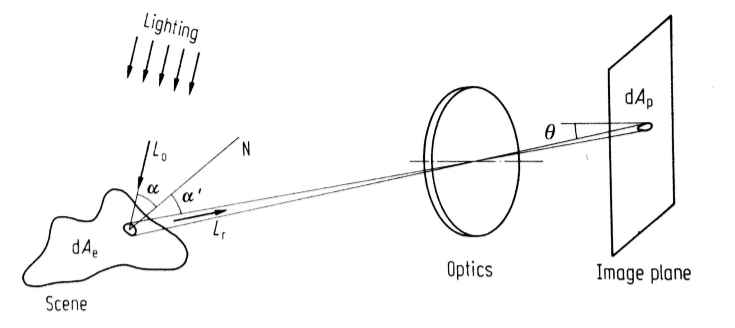
\includegraphics[width =130mm]{fig1_1} \\
		\textbf  {Figura 1.1} Formarea imaginii
	\end {footnotesize} 
\end {center}
\tab Sistemul vizual uman este unul complex din punct de vedere al puterii lui de analiză a imaginilor digitale, având capacitatea de a separa în mod corect obiectele dintr-o imagine de
fundalul acesteia. De exemplu, se pot obține informații despre forma și transparența unei patale în diverse faze ale sursei de lumină, dar și comparativ cu fundalul imaginii din care floarea
face parte (figura 1.2).
\newline
\begin {center} 
	\begin {footnotesize} 
		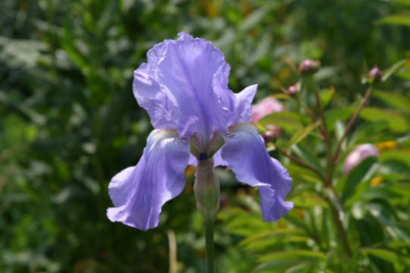
\includegraphics[width = 80mm]{fig1_2} \\
		\textbf  {Figura 1.2} Sistemul vizual uman partiționează imaginea în \\ mai două segmente: floare, respectiv fundal
	\end {footnotesize} 
\end {center}
\tab De-a lungul timpului, psihologii au încercat să descopere modul în care funcționează sistemul vizual uman. În urma cercetărilor realizate s-a ajuns la concluzia că domeniul vederii artificiale
poate acoperi cu o mai mare exactitate o anumită arie a imaginilor digitale. 
\newline \tab Se vor analiza o serie de iluzii optice care demonstrează faptul că în anumite condiții aplicațiile din domeniul vederii artificiale dau un răspuns sigur în urma procesării imaginilor digitale, comparativ
cu sistemul vizual uman care întâmpină anumite dificultăți. \\ \tab În figura 1.3 se prezintă iluzia clasică Muller-Lyer, unde cele două linii orizontale par a avea lungimi diferite, probabil din cauza 
efectelor de perpectivă diferite.  
\newline
\begin {center} 
	\begin {footnotesize} 
		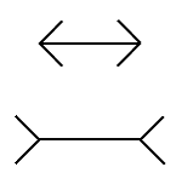
\includegraphics[width = 40mm]{fig1_3} \\
		\textbf  {Figura 1.3} 
	\end {footnotesize} 
\end {center}
\tab În figura 1.4 se prezintă iluzia optică a pătratului ``alb`` B aflat în umbră și a pătratului ``negru`` A aflat în lumină, care par a avea intensități diferite, însă acestea au intensități identince. 
\newline
\begin {center} 
	\begin {footnotesize} 
		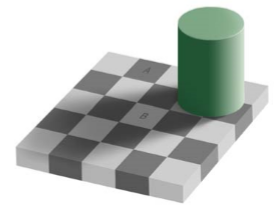
\includegraphics[width = 57mm]{fig1_4} \\
		\textbf  {Figura 1.4} 
	\end {footnotesize} 
\end {center}
\tab În figura 1.5 vom analiza pozițiile pe care se află x-urile roșii în partea din stângă, comparativ cu pozițiile lor în partea din dreapta. Se observă că este mult mai ușor de numărat de x-urile
roșii din partea stângă decât din partea dreaptă, fapt cauzat de un răspuns ``instantaneu`` dat de asocierile între culori pe care le face creierul uman. 
\newline
\begin {center} 
	\begin {footnotesize} 
		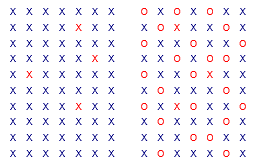
\includegraphics[width = 65mm]{fig1_5} \\
		\textbf  {Figura 1.5} 
	\end {footnotesize} 
\end {center}
\tab În concluzie, pentru un anumit tip de aplicații sistemul vizual uman oferă un răspuns mult mai precis, dar și mult mai rapid decât un sistem care integrează vederea artificială. De multe ori însă, un mod
mai ușor de procesare și analizare al unui set mare de imagini digitale este oferit de către un sistem de vedere artificială antrenat într-un anumit scop pentru a oferi un răspuns cât se poate de precis. 


\chapter{ Python}
\tab Aplicația de corectare automată a testelor grilă care este descrisă în prezenta lucrare a fost dezvoltată cu ajutorul limbajului de programare
Python. Python este utilizat pentru o mare varietate de aplicații, fiind astfel un limbaj de programare uzual, proiectat de Guido van
Rossum și dezvoltat de compania Python Software Foundation. Unul dintre avantajele importante ale utilizării acestui limbaj de programare este
acela ca Python este un limbaj de scripting, astfel încât codul scris se interpretează, nu se compliează, fapt care generează un timp redus în 
dezvoltarea și testarea aplicațiilor. Paradigmele de programare (prin paradigmă a se înțelege modul în care putem clasifica limbajele de programare),
pe care le adoptă limbajul Python sunt următoarele:
	\begin{enumerate}
	\setlength\itemsep{1pt}
	\item orientată obiect -  bazată pe conceptul de obiect care conține date, sub formă de câmpuri (atribute) și proceduri (metode)
	\item imperativă - bazată pe o execuție secvențială a intrucțiunilor care modifică starea programului
	\item funcțională - bazată pe aplicarea de funcții, astfel încât calculele devin o evaluare de funcții matematice
	\item procedurală - bazată pe apeluri de proceduri definite anterior, fiind similara cu paradigma funcțională
	\item reflectivă - bazată pe capacitatea unui program de a-și schimba stuctura și comportamentul în timpul execuției acestuia.
	\end{enumerate}
\tab Aplicația de corectare automată a testelor grilă a fost realizată în mediul de dezvoltare PyCharm, dezvoltat de compania cehă JetBrains, fiind 
un mediu specializat care oferă funcționalități de analiză a codului, testare unitară, integrare cu sisteme de gestionare a mai multor versiuni ale unei
aplicații, dezvoltare de aplicații web folosind Django. Fișierele dezvoltate în Python se numesc scripturi și au extensia ``.py``. Un aspect important
este faptul că un proiect realizat în PyCharm este stucturat în mai multe fișiere cu extensia ``.py``, definite ca module. Un modul poate importa
alte module, astfel încât aceste importuri trebuie realizate la începutul unui script sau modul. Fiecare modul are definit un tabel de simboluri, în care
se vor salva informații despre variabilele folosite în script, dar și numele modulelor importate de acesta. În cazul importării fară a se utiliza un anumit modul,
se va primit un mesaj de atenționare (s-a efectuat o importare a unui modul care nu se folosește).
\newline
\tab Stuctura de date de bază utilizată în aplicație este reprezentată de matrice, motivul fiind faptul că imaginile au o structura matriceala. Pentru 
o imagine în tonuri de alb și negru, adică o imagine binară, se poate folosi o matrice bidimensională, în care fiecare pixel are o valoare de 0, adica negru 
sau 1, adica alb. Pentru o imagine în tonuri de gri se poate folosi o matrice bidimensională, în care fiecare pixel are o valoare între 0 și 255, unde 0 
înseamnă negru, 255 înseamnă alb, iar 127 cea mai bună nuanță de gri. Pentru imaginile color se poate folosi o matrice tridimensională, pentru că
se dorește o reprezentare RGB (Red Green Blue), motiv pentru care fiecare pixel reprezintă o combinație din intensitatea canalului roșu (Red), a celui
verde (Green) și a celui albastru (Blue). Pentru a obține o imagine în tonuri de gri dintr-o imagine color, fiecare pixel care aparține imaginii în 
tonuri de gri va avea o valoare calculată folosind formula următoare: $x=0.299*r+0.587*g+0.114*b$, unde r, g, b sunt valorile fiecărui canal în parte, care 
aparțin pixelului color, iar x este valoarea rezultată care va fi atribuită pixelului din imaginea în tonuri de gri.
\newline
\tab În dezvoltarea aplicației descrisă în această lucrare s-au utilizat următoarele module pe care limbajul Python le poate importa:
	\begin{enumerate}
	\setlength\itemsep{1pt}
	\item NumPy
	\item Tkinter
	\item UnitTest
	\item OpenCV
	\item TensorFlow
	\end{enumerate}
\tab Rolul acestor module urmează a fi explicat în continuare.

\section {NumPy}
\tab Modulul NumPy (Numerical Python) este o extensie care aparține limbajului Python, având ca scop fundamental manipularea unor stucturi de date de dimensiuni 
mari, printre care mulțimile de elemente (arrays) și matricile (matrices), dar și o varietate de funcții matematice de nivel înalt care operează peste aceste structuri de date. Obiectul principal folosit
de către acest modul este o mulțime multidimensională, definită sub forma unui tabel de elemente (de obicei numere), toate având același tip de date, indexată 
folosind un tuplu format din numere întregi, pozitive. În NumPy, dimensiunile unui vector sau ale unei matrice poartă denumirea de \textit{axe}, iar numărul total al acestora
se numește \textit{rang}.
\newline\tab\textbf{ Exemplu 1:} Coordonatele unui punct într-un spațiu 3D, [1, 2, 1] este o mulțime care are rangul 1, deoarece are o singură axă, iar aceasta are dimensiunea 3. 
\newline\tab\textbf{ Exemplu 2:} Mulțimea [[1., 0., 0.], [0., 1., 2.]] are rangul egal cu 2, fiind astfel o mulțime de elemente bidimensională. Prima dimensiune, adică prima axă are lungimea 2,
iar cea de-a doua dimensiune are lungimea 3.
\newline
\newline\tab Clasa care aparține modulului NumPy, și care are rolul de a manipula mulțimile se numește \textit{ndarray}. Printre cele mai importante câmpuri ale unui obiect de tipul ndarray se află:
\newline - \textit{ndarray.ndim} - reprezentând numărul de axe (dimensiuni) ale mulțimii (echivalentul rang-ului unei mulțimi)
\newline - \textit{ndarray.shape} - tuplul de numere întregi pozitive care reprezintă
dimensiunea fiecărei axe a mulțimii (pentru o matrice de \textit {n rânduri} și \textit {m coloanei} valoarea tupului va fi (n,m)
\newline - \textit {ndarray.size} - numărul total de elemente ale mulțimii, având o valoare egală cu produsul elementelor întregi din tuplul returnat de câmpul shape.

\section{Tkinter}
\tab Modulul Tkinter este o bibliotecă standard, creată pentru limbajul de programare Python, necesară pentru crearea interfețelor grafice dintre utilizator și mașina care 
găzduiește o anumită aplicație.  Python, alături de Tkinter, oferă programatorului un mod ușor și intuitiv pentru crearea unei interfețe grafice care să ofere o anumită 
funcționalitate utilizatorului (se folosește o paradigmă orientată obiect). 
\newline\tab Pașii care trebuie parcurși pentru crearea unei interfețe grafice în Python sunt:
\newline - importarea modulului \textit {tkinter}
\newline - crearea ferestrei principale a aplicației (cea care se va deschide prima dată în momentul rulării aplicației)
\newline - adăugarea unor componente interfeței (butoane, câmpuri în care se poate introduce text)
\newline - adăugarea unui eveniment care poartă denumirea de ``mainloop``, cu scopul de a acționa în momentul în care utilizatorul folosește o anumită componentă adăugată în interfață.

\section{UnitTest}
\tab Modulul UnitTest este biblioteca standard pentru testare unitară a aplicațiilor scrise în Python, deseori găsindu-se sub denumirea de ``PyUnit``, dezvoltată de Kent Beck și Erich Gamma. 
Acest modul oferă o listă de clase care permit efectuarea testelor automate asupra aplicației, partajarea unor setări speciale pentru pornirea sau oprirea testelor, agregarea unor teste într-o 
anumită colecție (spre exemplu crearea unei suite de teste pe baza claselor de echivalență existente în cadrul unei aplicații).
\newline\tab Pentru o bună funcționare a activității de testare, modulul UnitTest oferă câteva concepte importante, care interconectate, conduc la realizarea cu ușurință a acestei componente 
importante din dezvoltarea unei aplicații software:
\newline - pregătirea testului: reprezintă activitatea premergătoare testării propriu-zise. În unele cazuri poate conduce la curățarea unor baze de date de test, crearea unor noi baze de date sau 
a unor directoare noi.
\newline - cazuri de testare: reprezintă cea mai mică unitate de testare, folosită pentru a determina răspunsul unei componente a aplicației pentru un caz particular de parametrii. Modulul UnitTest
oferă o clasă de bază, TestCase, care se utilizează în momentul creării unui caz de testare.
\newline - suită de teste: reprezintă o colecție de cazuri de testare sau chiar o colecție de suite de teste. Scopul acesteia este de a agrega testele care trebuie executate împreună.
\newline - componenta care execută testele și oferă răspuns imediat programatorului. Se oferă informații cu privire la testele care s-au rulat, alături de rezultatele acestora.

\section{OpenCV}
\tab Modulul OpenCV(Open Source Computer Vision) este o bibliotecă folosită în dezvoltarea aplicațiilor de vedere artificială. Dezvoltarea acestui modul, de către Gary Bradsky, a început în anul 1999 la Intel,
iar prima variantă a fost finalizată în anul 2000. În prezent, OpenCV suportă o varietate de algortmi din domeniul vederii artificiale, dar și al machine learning-ului.
\\ \tab OpenCV-Python este API-ul corespunzător bibliotecii standard de OpenCV, care combină modulul de vedere artificială din limbajul C++ și limbajul Python.

\section{TensorFlow}
\tab TensorFlow este o bibliotecă open source folosită pentru operații de calcul științific, unde datele sunt reprezentate sub forma unui graf. 
Această bibliotecă este folosită în dezvoltarea aplicațiilor de \textit{machine learning}, dezvoltată de către cei de la Google pentru crearea, antrenarea 
rețelelor neurale cu scopul de a detecta și descifra modele similare cu cele ale gândirii umane.
\\ \tab Machine learning este un subdomeniu al informaticii, care după definiția lui Arthur Samuel din 1959 reprezintă ``abilitatea mașinilor de calcul de a învăța și reproduce o anumită funcționalitate
fară a fi programată în acest sens``. Printre aplicațiile acestui subdomeniu se regăsesc filtrarea email-urilor, detectarea răufăcătorilor dintr-o rețea, detectarea caracterelor dintr-o imagine (OCR - Optical Character 
Recognition). 
\\ \tab Graful sub care sunt reprezentate datele are nodurile reprezentate de operațiile matematice, iar muchiile
de vectori multidimensionali care se numesc tensori. Se definește \textit{rang-ul} unui tensor dimensiunea acestuia. De exemplu, tensorul [1, 2, 3] este un vector cu rang-ul 3. 

\chapter{Implementare}

\tab Lucrarea de față propune un algoritm de corectare a testelor grilă care au un format prezentat în figura 2.1. Subiectele primite de către elevi sunt structurate în 4 tipuri de variante (numerotate de la 1 la 4), 
fiecare având un subiect de matematică, unul de informatică și unul de fizică. Grila de matematică este obligatorie, iar dintre grilele de fizică și informatică elevul trebuie sa rezolve una. În funcție de tipul grilei pe care elevul
decide să o rezolve, se va trece numărul corespunzător acesteia (1, 2, 3 sau 4) în căsuța de fizică sau informatică, după cum urmează: dacă un elev primește varianta 2 și alege să rezolve grila de fizică, se va completa numărul 2
în dreptul opțiunii dorite (figura 2.2).
\newline
\begin {center} 
	\begin {footnotesize} 
		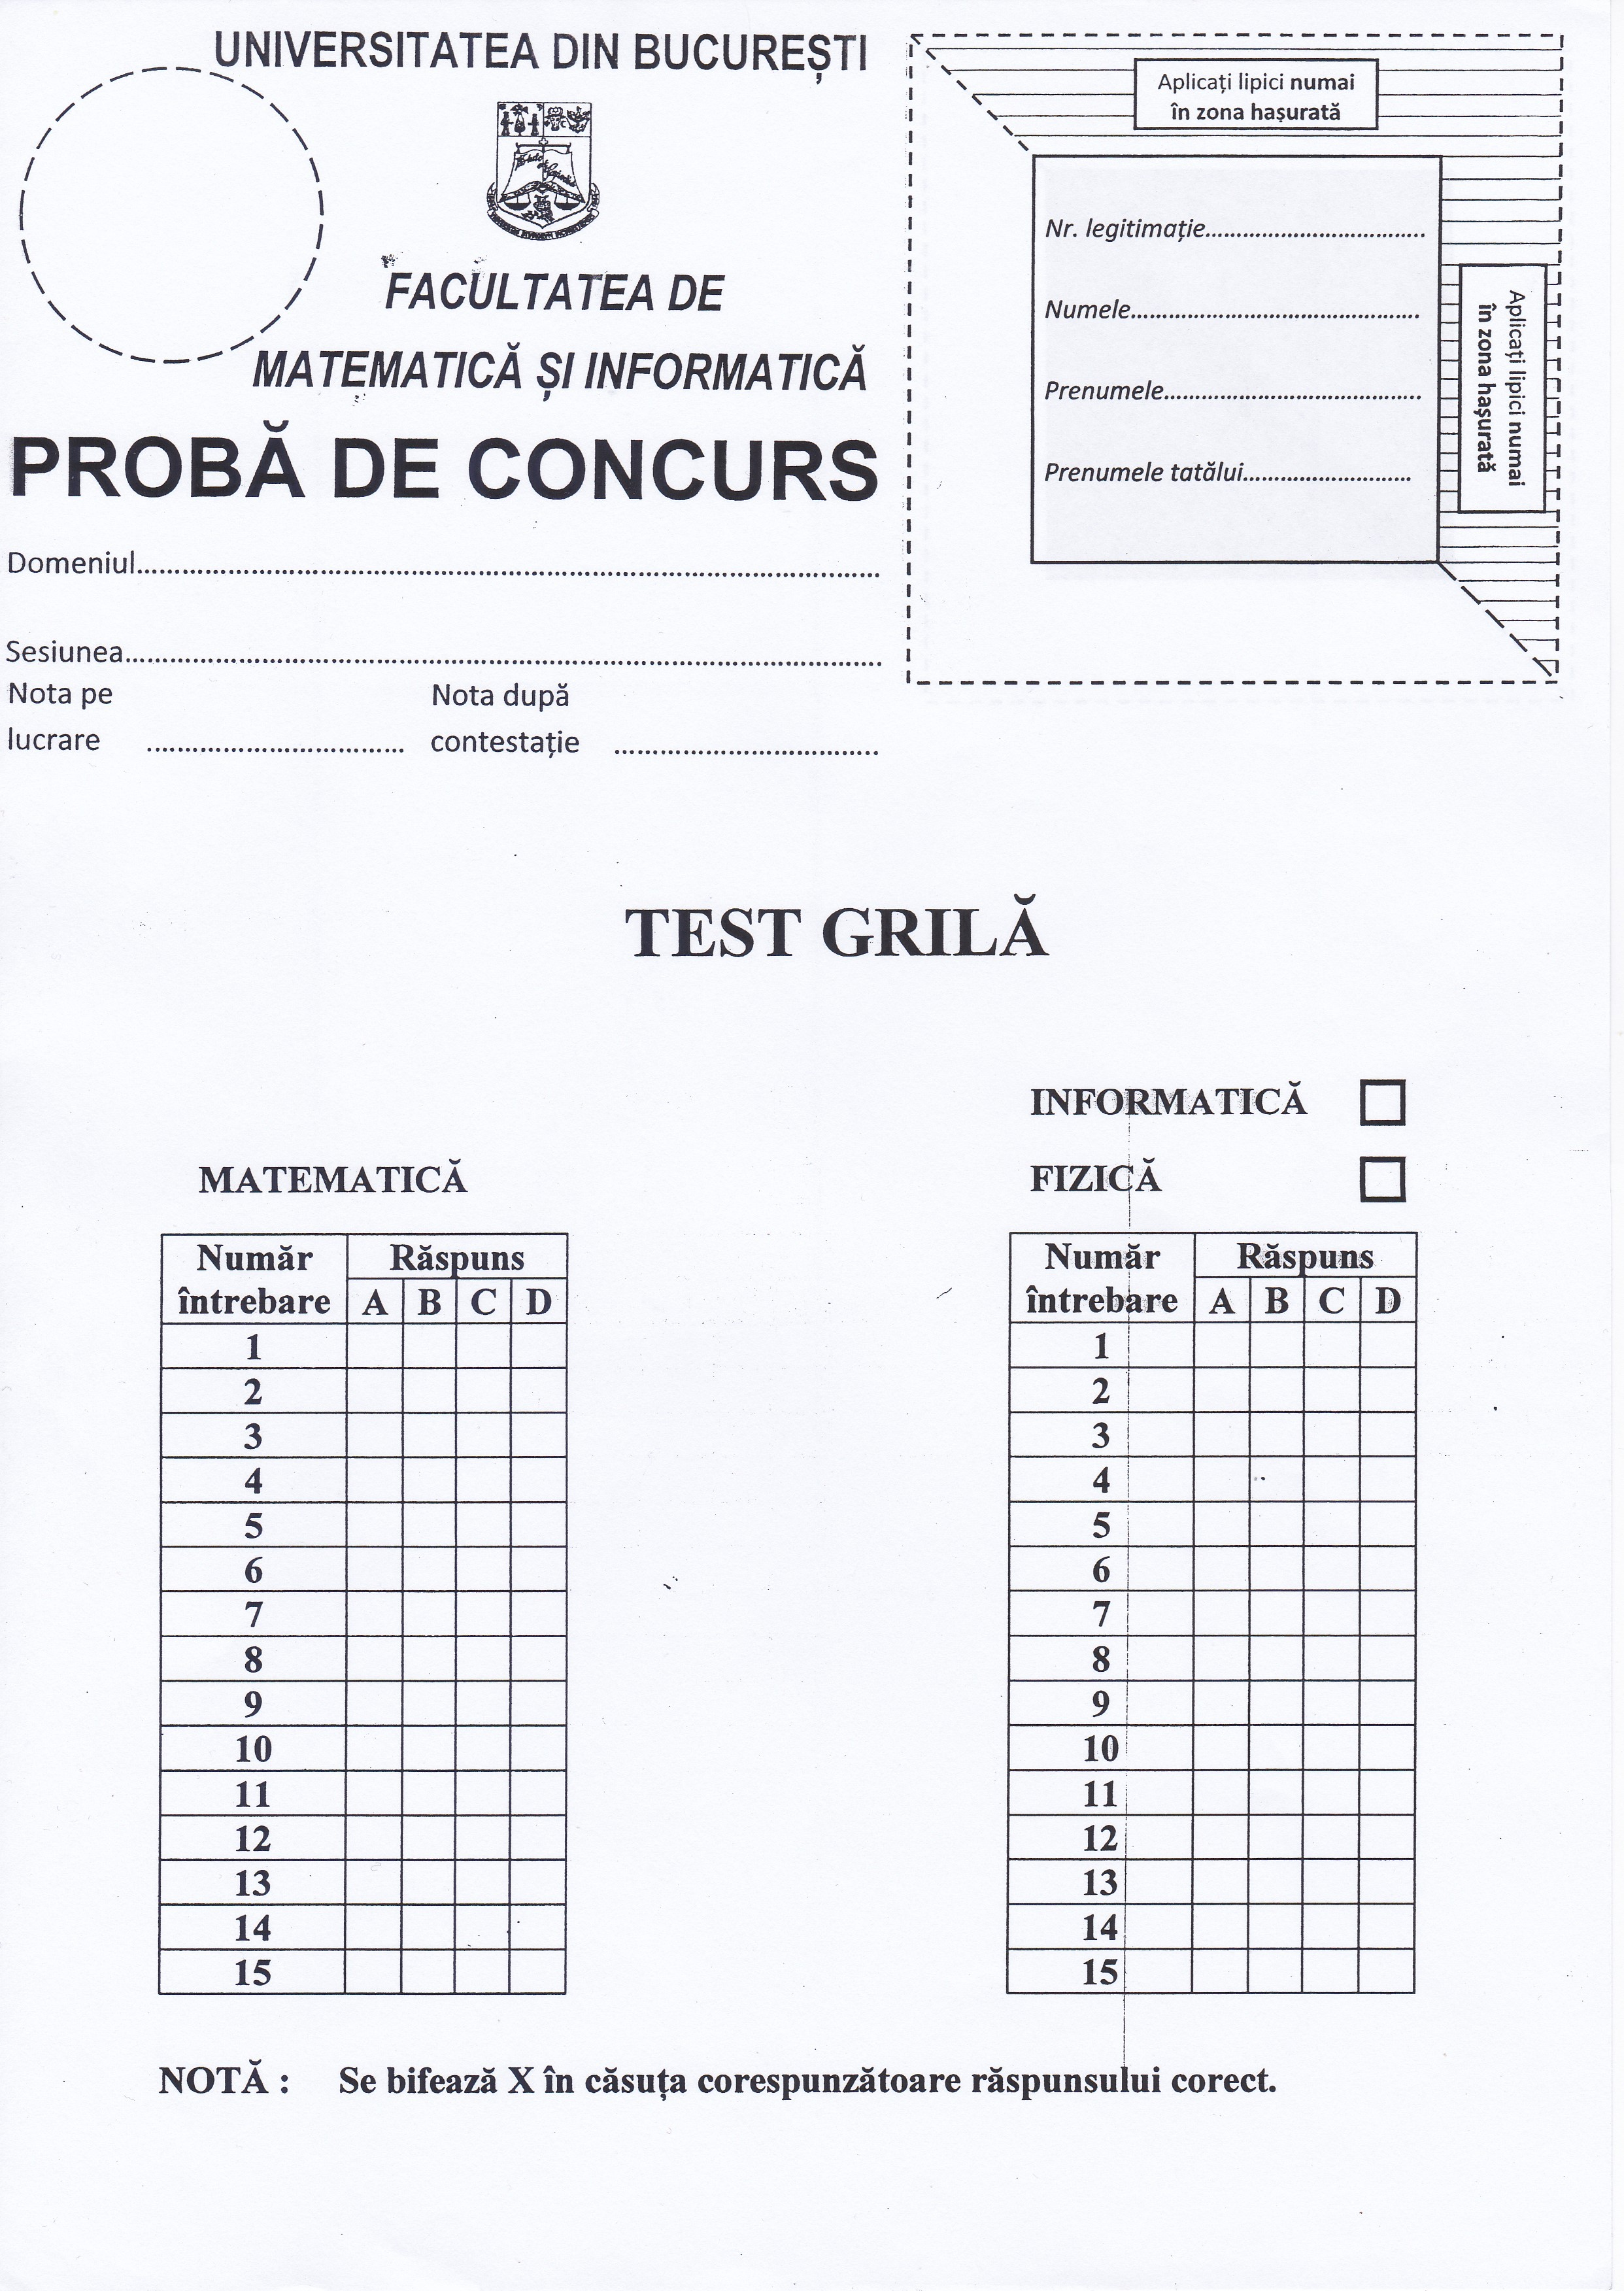
\includegraphics[width = 70mm]{fig2_1} \\
		\textbf  {Figura 2.1} 
	\end {footnotesize} 
\end {center}

\begin {center} 
	\begin {footnotesize} 
		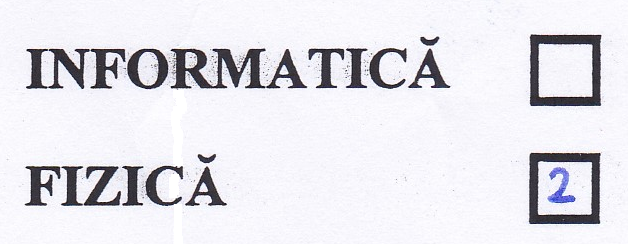
\includegraphics[width = 40mm]{fig2_2} \\
		\textbf  {Figura 2.2} 
	\end {footnotesize} 
\end {center}


\tab Corectarea unui set de teste completate de către elevi se bazeză pe următorul scenariu:
	\begin{enumerate}
	\setlength\itemsep{1pt}
	\item scanarea tuturor testelor elevilor și salvarea acestora într-un anumit director
	\item introducerea răspunsurilor corecte de către comisia de admitere în aplicație
	\item pregătirea imaginii pentru a fi procesată - eliminarea zgomotului care apare în urma printării și scanării acesteia
	\item găsirea în imagine a celor două grile existente
	\item determinarea răspunsurilor bifate de către elev 
	\item determinarea tipului de grilă la care elevul a răspuns (fizică sau informatică), dar și a numărului acestei grile (1, 2, 3 sau 4)
	\item compararea răspunsurilor bifate de către elev cu cele introduse de către comisia de admitere
	\item determinarea notei finale care se bazează pe formula: Nota finală = 0.3p *  numărul răspunsurilor corecte + 1p (oficiu). 
	\end{enumerate}

\section{Pasul 1}
\tab Scanarea tuturor lucrărilor completate de către elevi se va face cu ajutorul unui scanner, iar în urma acestui proces imaginile se vor salva într-un director.
 
\section{Pasul 2}
\tab Înterfața grafică a aplicației descrise în prezenta lucrare conține o funcționalitate de adăugare a răspunsurilor corecte. Comisia de admitere accesează această funcționalitate, introducând valoarea 1 pe poziția pe care răspunsul corect 
la o anumită întrebare, respectiv 0 pentru cele 3 poziții incorecte (figura 2.3). De asemenea, se va alege tipul grilei pentru care se vor introduce rezultatele la un anumit moment (exemplu: Matematica 1 - reprezintă grila corespunzătoare variantei 1).
\begin {center} 
	\begin {footnotesize} 
		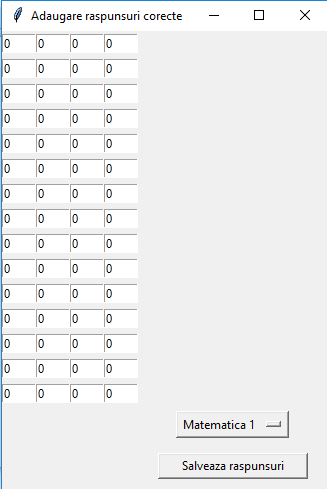
\includegraphics[width = 55mm]{fig2_3}
		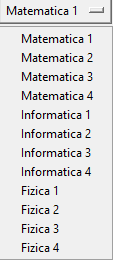
\includegraphics[width = 27mm]{fig2_4} \\
		\textbf  {Figura 2.3} 
	\end {footnotesize} 
\end {center}

\section{Pasul 3}
\tab Pregătirea imaginii pentru a fi procesată este un pas foarte important, adăugat în prezenta lucrare după primele rezultate ale detectării grilelor existente în pagină. Datorită imprimării grilelor, dar și a scanării acestora este inevitabil ca imaginile 
rezultate să nu aibă zgomot. Drept urmare acest pas este unul util în vederea detectării corecte a informațiilor dorite.
\\ \tab Eliminarea zgomotului din imaginile rezultate a fost realizată prin definirea unui modul care conține 4 metode:
\\ - prepareImage(img): metodă care primește ca parametru o imagine pe care o transformă din imagine RGB în imagine în tonuri de gri, aplicându-i un filtru de blurare și returnează imaginea ``outputSmooth.jpg``
\\ - removeNoiseByPixel(img, column, line, passFactor: care primește ca parametru o imagine, pozițiile unui pixel în imagine (coloană, rând) și o valoare numerică între 0 - 255. Rezultatul acestei metode este o imagine în care pixelii cu o intensitate
sub valoarea lui passFactor devind 0 (pixeli negri), iar cei cu o intensitate peste valoarea lui passFactor devin 255 (pixeli albi).
\\ - removeNoise(img, passFactor):  metodă care primește ca parametru o imagine și o valoare numerică între 0 - 255, va parcurge fiecare pixel al imaginii, apelând metoda removeNoiseByPixel
\\ - removeNoiseMain(imgName, passFactor): metoda principală a modulului, care citește imaginea, o redimensionează pentru ca timpul procesării să fie mai mic și apelează pentru imaginea citiă metodele prepareImage și
removeNoise. Rezultatul imaginii se va numi ``noiseRemoved.jpg``.
\\ \tab În urma pregătirii imaginii pentru a fi procesată se observă rezultatul aplicării metodei removeNoiseMain asupra imaginii inițiale:
\begin {center} 
	\begin {footnotesize} 
		\textbf  {1. Imaginea inițială} 
		\\
		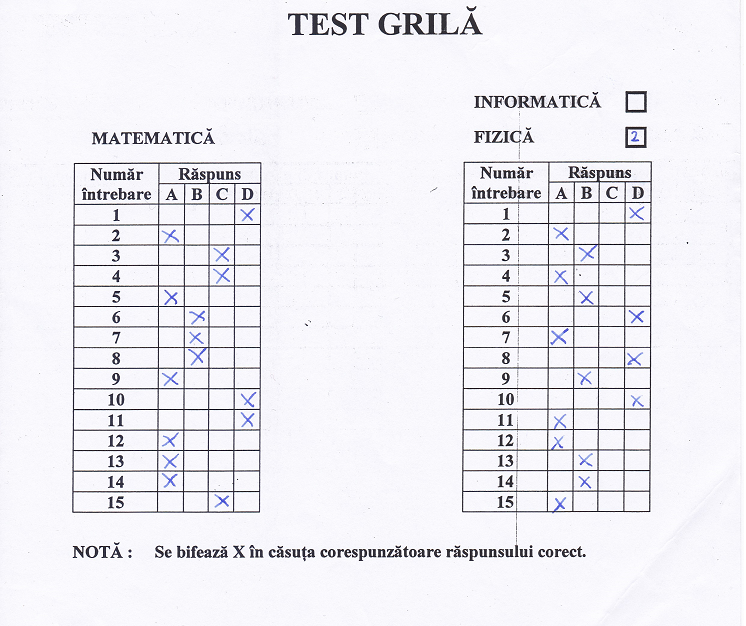
\includegraphics[width = 75mm]{fig2_5}
		\\ 
		\textbf  {2. Imaginea noiseRemoved} 
		\\
		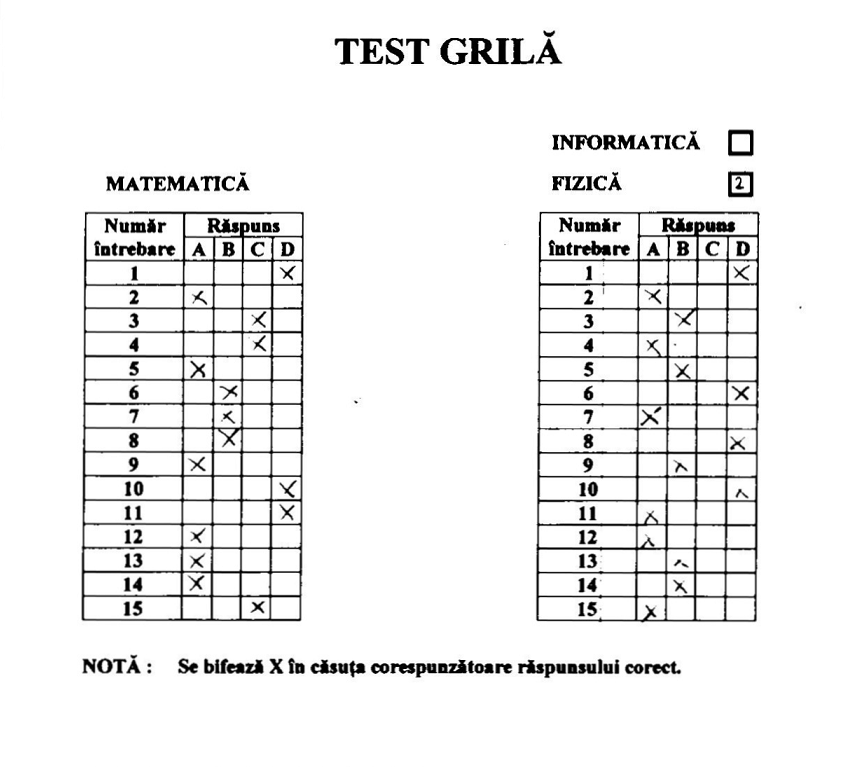
\includegraphics[width = 75mm]{fig2_7}
		
	\end {footnotesize} 
\end {center}

\section{Pasul 4}
\tab Găsirea în imagine a celor două grile existente implică definirea mai multor module în aplicația descrisă în prezenta lucrare. 
\\ \tab Un prim modul este findTest, în care se definește o metodă cu aceeași denumire care primește ca parametru numele unei imagini. Metoda parcurge următorii pași:


\end{document}





















